% This is a modified version of the tufte-latex book example in which the title page and the contents page resemble Tufte's VDQI book, using Kevin Godby's code from this thread at https://groups.google.com/forum/#!topic/tufte-latex/ujdzrktC1BQ.
%% Unfortunately for the contents to contain
%% the "Parts" lines successfully, hyperref
%% needs to be disabled.
\documentclass[nohyper,nobib,a4paper]{tufte-book}
\usepackage{nameref}
\usepackage{algorithm} %Note: remove if errors
%\usepackage{algorithmic} %Note: remove if errors
\usepackage{algpseudocode}
\usepackage[dutch]{babel}
\usepackage{csquotes}

% \hypersetup{colorlinks}% uncomment this line if you prefer colored hyperlinks (e.g., for onscreen viewing)
%
\usepackage{ dsfont } % for fancy Z and R and N 
\usepackage{amsmath}
\DeclareMathOperator\supp{supp}
\DeclareMathOperator\conf{conf}
\DeclareMathOperator\MIS{MIS}
%
% \usepackage{hyphenat}
\usepackage{url}
\usepackage{xargs}

\renewcommandx{\cite}[3][1={0pt},2={}]{\sidenote[][#1]{\fullcite[#2]{#3}}}

%%
% Book metadata
\title{Optimalisatietechnieken}
\date{}
\author[Pieter Delobelle Anton Danneels]{Pieter Delobelle \\ Anton Danneels}
\publisher{KU Leuven}

%%
% If they're installed, use Bergamo and Chantilly from www.fontsite.com.
% They're clones of Bembo and Gill Sans, respectively.
%\IfFileExists{bergamo.sty}{\usepackage[osf]{bergamo}}{}% Bembo
%\IfFileExists{chantill.sty}{\usepackage{chantill}}{}% Gill Sans

%\usepackage{microtype}

%%
% Just some sample text
\usepackage{lipsum}

%%
% For nicely typeset tabular material
\usepackage{booktabs}

%%
% For graphics / images
\usepackage{graphicx}
\setkeys{Gin}{width=\linewidth,totalheight=\textheight,keepaspectratio}
\graphicspath{{graphics/}}

% The fancyvrb package lets us customize the formatting of verbatim
% environments.  We use a slightly smaller font.
\usepackage{fancyvrb}
\fvset{fontsize=\normalsize}

%%
% Prints argument within hanging parentheses (i.e., parentheses that take
% up no horizontal space).  Useful in tabular environments.
\newcommand{\hangp}[1]{\makebox[0pt][r]{(}#1\makebox[0pt][l]{)}}

%%
% Prints an asterisk that takes up no horizontal space.
% Useful in tabular environments.
\newcommand{\hangstar}{\makebox[0pt][l]{*}}

%%
% Prints a trailing space in a smart way.
\usepackage{xspace}

%\usepackage{amsmath}

%%
% Some shortcuts for Tufte's book titles.  The lowercase commands will
% produce the initials of the book title in italics.  The all-caps commands
% will print out the full title of the book in italics.
\newcommand{\vdqi}{\textit{VDQI}\xspace}
\newcommand{\ei}{\textit{EI}\xspace}
\newcommand{\ve}{\textit{VE}\xspace}
\newcommand{\be}{\textit{BE}\xspace}
\newcommand{\VDQI}{\textit{The Visual Display of Quantitative Information}\xspace}
\newcommand{\EI}{\textit{Envisioning Information}\xspace}
\newcommand{\VE}{\textit{Visual Explanations}\xspace}
\newcommand{\BE}{\textit{Beautiful Evidence}\xspace}

\newcommand{\TL}{Tufte-\LaTeX\xspace}

% Prints the month name (e.g., January) and the year (e.g., 2008)
\newcommand{\monthyear}{%
  \ifcase\month\or January\or February\or March\or April\or May\or June\or
  July\or August\or September\or October\or November\or
  December\fi\space\number\year
}


% Prints an epigraph and speaker in sans serif, all-caps type.
\newcommand{\openepigraph}[2]{%
  %\sffamily\fontsize{14}{16}\selectfont
  \begin{fullwidth}
  \sffamily\large
  \begin{doublespace}
  \noindent\allcaps{#1}\\% epigraph
  \noindent\allcaps{#2}% author
  \end{doublespace}
  \end{fullwidth}
}

% Inserts a blank page
\newcommand{\blankpage}{\newpage\hbox{}\thispagestyle{empty}\newpage}

\usepackage{units}

% Typesets the font size, leading, and measure in the form of 10/12x26 pc.
\newcommand{\measure}[3]{#1/#2$\times$\unit[#3]{pc}}

% Macros for typesetting the documentation
\newcommand{\hlred}[1]{\textcolor{Maroon}{#1}}% prints in red
\newcommand{\hangleft}[1]{\makebox[0pt][r]{#1}}
\newcommand{\hairsp}{\hspace{1pt}}% hair space
\newcommand{\hquad}{\hskip0.5em\relax}% half quad space
\newcommand{\TODO}{\textcolor{red}{\bf TODO!}\xspace}
\newcommand{\ie}{\textit{i.\hairsp{}e.}\xspace}
\newcommand{\eg}{\textit{e.\hairsp{}g.}\xspace}
\newcommand{\na}{\quad--}% used in tables for N/A cells
\providecommand{\XeLaTeX}{X\lower.5ex\hbox{\kern-0.15em\reflectbox{E}}\kern-0.1em\LaTeX}
\newcommand{\tXeLaTeX}{\XeLaTeX\index{XeLaTeX@\protect\XeLaTeX}}
% \index{\texttt{\textbackslash xyz}@\hangleft{\texttt{\textbackslash}}\texttt{xyz}}
\newcommand{\tuftebs}{\symbol{'134}}% a backslash in tt type in OT1/T1
\newcommand{\doccmdnoindex}[2][]{\texttt{\tuftebs#2}}% command name -- adds backslash automatically (and doesn't add cmd to the index)
\newcommand{\doccmddef}[2][]{%
  \hlred{\texttt{\tuftebs#2}}\label{cmd:#2}%
  \ifthenelse{\isempty{#1}}%
    {% add the command to the index
      \index{#2 command@\protect\hangleft{\texttt{\tuftebs}}\texttt{#2}}% command name
    }%
    {% add the command and package to the index
      \index{#2 command@\protect\hangleft{\texttt{\tuftebs}}\texttt{#2} (\texttt{#1} package)}% command name
      \index{#1 package@\texttt{#1} package}\index{packages!#1@\texttt{#1}}% package name
    }%
}% command name -- adds backslash automatically
\newcommand{\doccmd}[2][]{%
  \texttt{\tuftebs#2}%
  \ifthenelse{\isempty{#1}}%
    {% add the command to the index
      \index{#2 command@\protect\hangleft{\texttt{\tuftebs}}\texttt{#2}}% command name
    }%
    {% add the command and package to the index
      \index{#2 command@\protect\hangleft{\texttt{\tuftebs}}\texttt{#2} (\texttt{#1} package)}% command name
      \index{#1 package@\texttt{#1} package}\index{packages!#1@\texttt{#1}}% package name
    }%
}% command name -- adds backslash automatically
\newcommand{\docopt}[1]{\ensuremath{\langle}\textrm{\textit{#1}}\ensuremath{\rangle}}% optional command argument
\newcommand{\docarg}[1]{\textrm{\textit{#1}}}% (required) command argument
\newenvironment{docspec}{\begin{quotation}\ttfamily\parskip0pt\parindent0pt\ignorespaces}{\end{quotation}}% command specification environment
\newcommand{\docenv}[1]{\texttt{#1}\index{#1 environment@\texttt{#1} environment}\index{environments!#1@\texttt{#1}}}% environment name
\newcommand{\docenvdef}[1]{\hlred{\texttt{#1}}\label{env:#1}\index{#1 environment@\texttt{#1} environment}\index{environments!#1@\texttt{#1}}}% environment name
\newcommand{\docpkg}[1]{\texttt{#1}\index{#1 package@\texttt{#1} package}\index{packages!#1@\texttt{#1}}}% package name
\newcommand{\doccls}[1]{\texttt{#1}}% document class name
\newcommand{\docclsopt}[1]{\texttt{#1}\index{#1 class option@\texttt{#1} class option}\index{class options!#1@\texttt{#1}}}% document class option name
\newcommand{\docclsoptdef}[1]{\hlred{\texttt{#1}}\label{clsopt:#1}\index{#1 class option@\texttt{#1} class option}\index{class options!#1@\texttt{#1}}}% document class option name defined
\newcommand{\docmsg}[2]{\bigskip\begin{fullwidth}\noindent\ttfamily#1\end{fullwidth}\medskip\par\noindent#2}
\newcommand{\docfilehook}[2]{\texttt{#1}\index{file hooks!#2}\index{#1@\texttt{#1}}}
\newcommand{\doccounter}[1]{\texttt{#1}\index{#1 counter@\texttt{#1} counter}}

% Generates the index
\usepackage{makeidx}
\makeindex

%%%% Kevin Godny's code for title page and contents from https://groups.google.com/forum/#!topic/tufte-latex/ujdzrktC1BQ
\makeatletter
\addto\captionsdutch{\renewcommand{\ALG@name}{Algoritme}}
\renewcommand{\maketitlepage}{%
\begingroup%
\setlength{\parindent}{0pt}

{\fontsize{24}{24}\selectfont\textit{\@author}\par}

\vspace{1.75in}{\fontsize{36}{54}\selectfont\@title\par}

\vspace{0.5in}{\fontsize{14}{14}\selectfont\textsf{\smallcaps{\@date}}\par}

\vfill{\fontsize{14}{14}\selectfont\textit{\@publisher}\par}

\thispagestyle{empty}
\endgroup
}
\makeatother

\titlecontents{part}%
    [0pt]% distance from left margin
    {\addvspace{0.25\baselineskip}}% above (global formatting of entry)
    {\allcaps{Part~\thecontentslabel}\allcaps}% before w/ label (label = ``Part I'')
    {\allcaps{Part~\thecontentslabel}\allcaps}% before w/o label
    {}% filler and page (leaders and page num)
    [\vspace*{0.5\baselineskip}]% after

\titlecontents{chapter}%
    [4em]% distance from left margin
    {}% above (global formatting of entry)
    {\contentslabel{2em}\textit}% before w/ label (label = ``Chapter 1'')
    {\hspace{0em}\textit}% before w/o label
    {\qquad\thecontentspage}% filler and page (leaders and page num)
    [\vspace*{0.5\baselineskip}]% after

\titlecontents{section}%
    [8em]% distance from left margin
    {}% above (global formatting of entry)
    {\contentslabel{2em}\textit}% before w/ label (label = ``section 1'')
    {\hspace{0em}\textit}% before w/o label
    {\qquad\thecontentspage}% filler and page (leaders and page num)
    [\vspace*{0.3\baselineskip}]% after
%%%% End additional code by Kevin Godby and Pieter Delobelle

\begin{document}

% Front matter
\frontmatter

% r.1 blank page
% \blankpage

% v.2 epigraphs
% \openepigraph{%
% A designer knows that he has achieved perfection 
% not when there is nothing left to add, 
% but when there is nothing left to take away.
% }{Antoine de Saint-Exup\'{e}ry}
% \vfill
% \openepigraph{%
% \ldots the designer of a new system must not only be the implementor and the first 
% large-scale user; the designer should also write the first user manual\ldots 
% If I had not participated fully in all these activities, 
% literally hundreds of improvements would never have been made, 
% because I would never have thought of them or perceived 
% why they were important.
% }{Donald E. Knuth}


% r.3 full title page
\maketitle


% v.4 copyright page
\newpage \thispagestyle{empty}
 \openepigraph{%
I have cleared the Augean stables of astronomy of cycles and spirals, and left behind me a single cartload of dung.
}{---Johannes Kepler%, {\itshape Design, Form, and Chaos}
}
 \vfill
\begin{fullwidth}
~\vfill
\thispagestyle{empty}
\setlength{\parindent}{0pt}
\setlength{\parskip}{\baselineskip}

\includegraphics[width=0.25\textwidth]{res/by-sa.eps}

\smallcaps{\the\year\ Pieter Delobelle}

\smallcaps{De inhoud van dit werk valt onder een Creative Commons Naamsvermelding-GelijkDelen 4.0 Internationaal-licentie}  (\url{https://creativecommons.org/licenses/by-sa/4.0}).


\par\smallcaps{Design by tufte-latex.googlecode.com, modifications by Pieter Delobelle}

\par The design is licensed under the Apache License, Version 2.0 (the ``License''); you may not
use this file except in compliance with the License. You may obtain a copy
of the License at \url{http://www.apache.org/licenses/LICENSE-2.0}. Unless
required by applicable law or agreed to in writing, software distributed
under the License is distributed on an \smallcaps{``AS IS'' BASIS, WITHOUT
WARRANTIES OR CONDITIONS OF ANY KIND}, either express or implied. See the
License for the specific language governing permissions and limitations
under the License.\index{license}

\end{fullwidth}

% r.5 contents
\setcounter{tocdepth}{1}
\tableofcontents

%\listoffigures

%\listoftables

% r.9 introduction
\cleardoublepage
\chapter*{Introductie}
Deze cursus hoort bij het vak \emph{optimalisatietechnieken} van Greet ..., gegeven op de Technologiecampus Gent van de Katholieke Universiteit van Leuven.

%%
% Start the main matter (normal chapters)
\mainmatter

% Chapter 1: Lineair en geheeltallig programmeren
\chapter{Heuristieken}

\subsection{Constructieve Heuristieken}

\subsection{Lokale zoekmethoden}

\subsection{Metaheuristieken}
%
%Chapter 2: Dynamisch programmeren
\chapter{fucking shit}
%
%Chapter 3: Branch and bound
\chapter{Branch and bound}

\section{Introductie}
\emph{Branch and bound} reduceert het aantal oplossingen dat in aanmerking komt door het probleem op te splitsen en suboptimale deeloplossingen te elimineren. 

\section{Parti\"ele oplossingen}
Door---bij een minimalisatieprobleem---gebruik te maken van een globale bovengrens en een ondergrens per knoop, is \emph{branch and bound} in staat om de takken die niet tot een optimale oplossing kunnen leiden te snoeien.

\paragraph{Bovengrens} Er wordt een globale bovengrens $UB$ bijgehouden, die verbetert per gevonden oplossing. 
Initieel is deze grens dus oneindig groot.

\paragraph{Ondergrens} Per knoop wordt een schatting gemaakt van de ondergrens $LB_i$.
Als deze ondergrens groter of gelijk is aan de bovengrens, $LB_i \geq UB$, dienden de kinderen van de node $i$ niet meer bekeken te worden.
Er is tenslotte geen mogelijkheid meer om een betere waarde te vinden dan de al gekende bovengrens.
%
%Chapter 4: Heuristieken en metaheuristieken
\chapter{Heuristieken en metaheuristieken}

\section{Introductie}
Heuristieken zijn informele methoden die \emph{voldoende goede} oplossingen kunnen opleveren voor complexe problemen. 
Hierbij worden twee soorten onderscheiden: constructieve en perturbatieve heuristieken.
Constructieve heuristieken bouwen een oplossing op en de groep van perturbatieve heuristieken maken wijzigingen aan een al bestaande oplossing.

\section{Modelleringen}
Een modellering dient om een oplossing voor te stellen, waarbij deze aan de volgende voorwaarden moet voldoen:

\begin{itemize}
    \item Volledigheid: alle mogelijke oplossingen kunnen voorgesteld worden in de modellering
    \item Connectiviteit: er bestaat een (indirect) pad tussen 2 oplossingen
    \item Effici\"entie: snel een eenvoudig te manipuleren en evalueren
\end{itemize}

\paragraph{Binaire codering}
Deze codering houdt voor ieder object een eigenschap bij. 
Bijvoorbeeld in geval van het knapzakprobleem, waarbij 0 voorstelt dat het item niet in de knapzak zit en 1 wel.
%
\begin{table}[!h]
    \centering
    \begin{tabular}{|l|l|l|l|l|l|l|}
    \hline
    1 & 0 & 0 & 1 & 1 & 1 & 0 \\ \hline
    \end{tabular}
\end{table}
%
\paragraph{Geheeltallige codering}
Deze codering kan meerdere eigenschappen toekennen aan een enkel object dan de binaire codering, wat voor toekennings- en locatieproblemen nuttig is.

Deze codering kan ook gebruikt worden om permutatie- en volgordeproblemen te weerspiegelen.
Hierbij kunnen nummers uiteraard geen twee keer voorkomen, tenzij de probleemstelling dat toelaat.
%
\begin{table}[!h]
    \centering
    \begin{tabular}{|l|l|l|l|l|l|l|}
    \hline
    4 & 7 & 8 & 1 & 2 & 6 & 5 \\ \hline
    \end{tabular}
\end{table}
%

\paragraph{Floating-point voorstelling}
Voor continue optimalisatieproblemen kan een voorstelling met zwevende komma's gebruikt worden.
Toepassingen zijn bijvoorbeeld het bepalen van samenstellingen of het optimaliseren vna parameters.

%
\begin{table}[!h]
    \centering
    \begin{tabular}{|l|l|l|l|l|l|l|}
    \hline
    2.5 & 0.8 & 10.3 & 1.0 & 2.3 & 4.6 & 0.1 \\ \hline
    \end{tabular}
\end{table}
%
\paragraph{Niet-lineaire voorstelling}
Mocht gekozen worden voor een niet-lineaire voorstelling van de oplossing, is dit in veel gevallen een graaf- of boomstructuur. 

\subsection{Directe en indirecte voorstelling}
Bij de modellering kan er gekozen worden om met een \emph{directe} voorstelling te werken, waarbij alle informatie direct beschikbaar is. Indien dit niet het geval is, en er dus een decoder nodig is om de oplossing te interpreteren, wordt gesproken van een \emph{indirecte} voorstelling.

\section{Lokale zoekmethoden}
Lokale zoekmethoden werken op basis van een initi\"ele oplossing, waarbij getracht wordt een lokaal minimum te bereiken. 
Deze algoritmen bestaan dus altijd uit twee stappen:

%
\begin{enumerate}
    \item Stap 1: construeer een initi\"ele oplossing.
    \item Stap 2: vervang de huidige oplossing door een betere buur.
\end{enumerate}
%

Het bepalen van een valide initi\"ele oplossing kan op verschillende manieren gebeuren. 
Zo kan er vertrokken worden van een al gekende oplossing. 
Een andere strategie is om met een eenvoudigere heuristiek of zelfs willekeurig een oplossing te genereren.


\section{Metaheuristieken}

%%
% The back matter contains appendices, bibliographies, indices, glossaries, etc.

%\backmatter

%	 \bibliography{sample-handout}
% \bibliographystyle{plainnat}


\end{document}

